\subsection{Iteration \#3}
I iteration 3 arbejdes med kamera blokken, som håndterer billedtagning, forsendelse af billeder og billede visning. Der monteres kamera på dronen, så den under flyvning kan tage billeder ved de GPS lokationer som bruger har defineret. Alle billeder der tages under flyvning sendes via mobilnet til server. Websiden henter automatisk de seneste billeder fra serveren og gør disse tilgængelige for bruger. Hvordan systemet er tiltænkt at bruges beskrives i user story nedenfor:

\subsubsection*{User story}
Under flyvning tager dronen billeder som sendes via 3G/GPS modulet til serveren. Websiden kontrollerer løbende hvilke billeder der er findes på serveren og gør disse tilgængelig for bruger. Login er påkrævet før bruger kan få lov at se information fra forskellige flyvninger.

%kommentar
\begin{figure}[H]
	\centering
	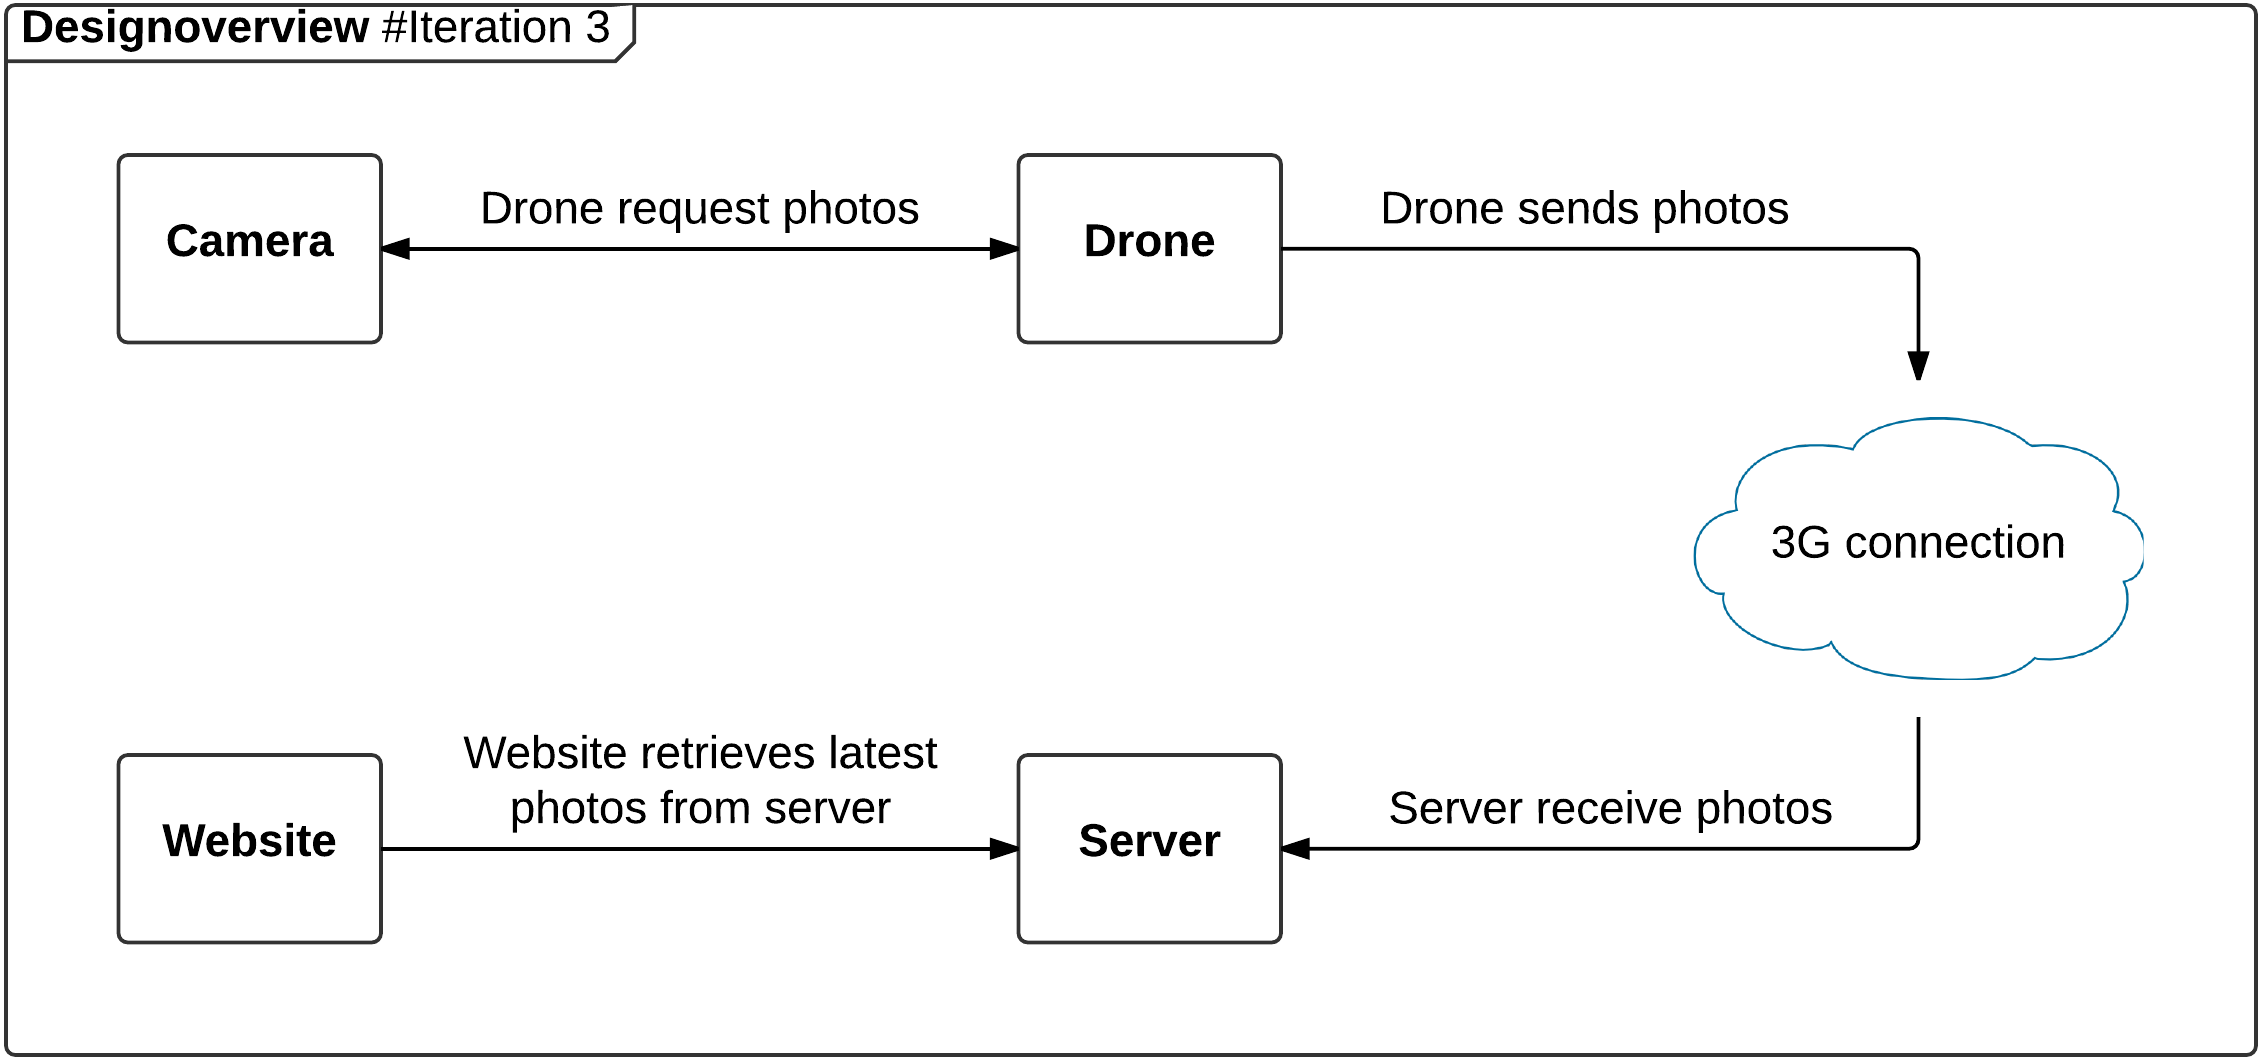
\includegraphics[width=1\textwidth]{Billeder/design_overview/design_overview_iteration3.png}
	\vspace{-.5cm}
	\caption{Designoverview \#iteration 3}
	\label{fig:design_overview_UC1}
\end{figure}
\newpage

\newpage
\subsubsection*{Pakkediagram drone}
I dette afsnit vises pakkediagram tilhørende drone. Hver pakke i pakkediagrammet består af en eller flere klasser, der med stort samspil udfører opgaver indenfor et fælles ansvarsområde. 
På hver pakke findes en lille beskrivelse, der tydeliggør pakkens ansvarsområde.

\begin{figure}[H]
	\centering
	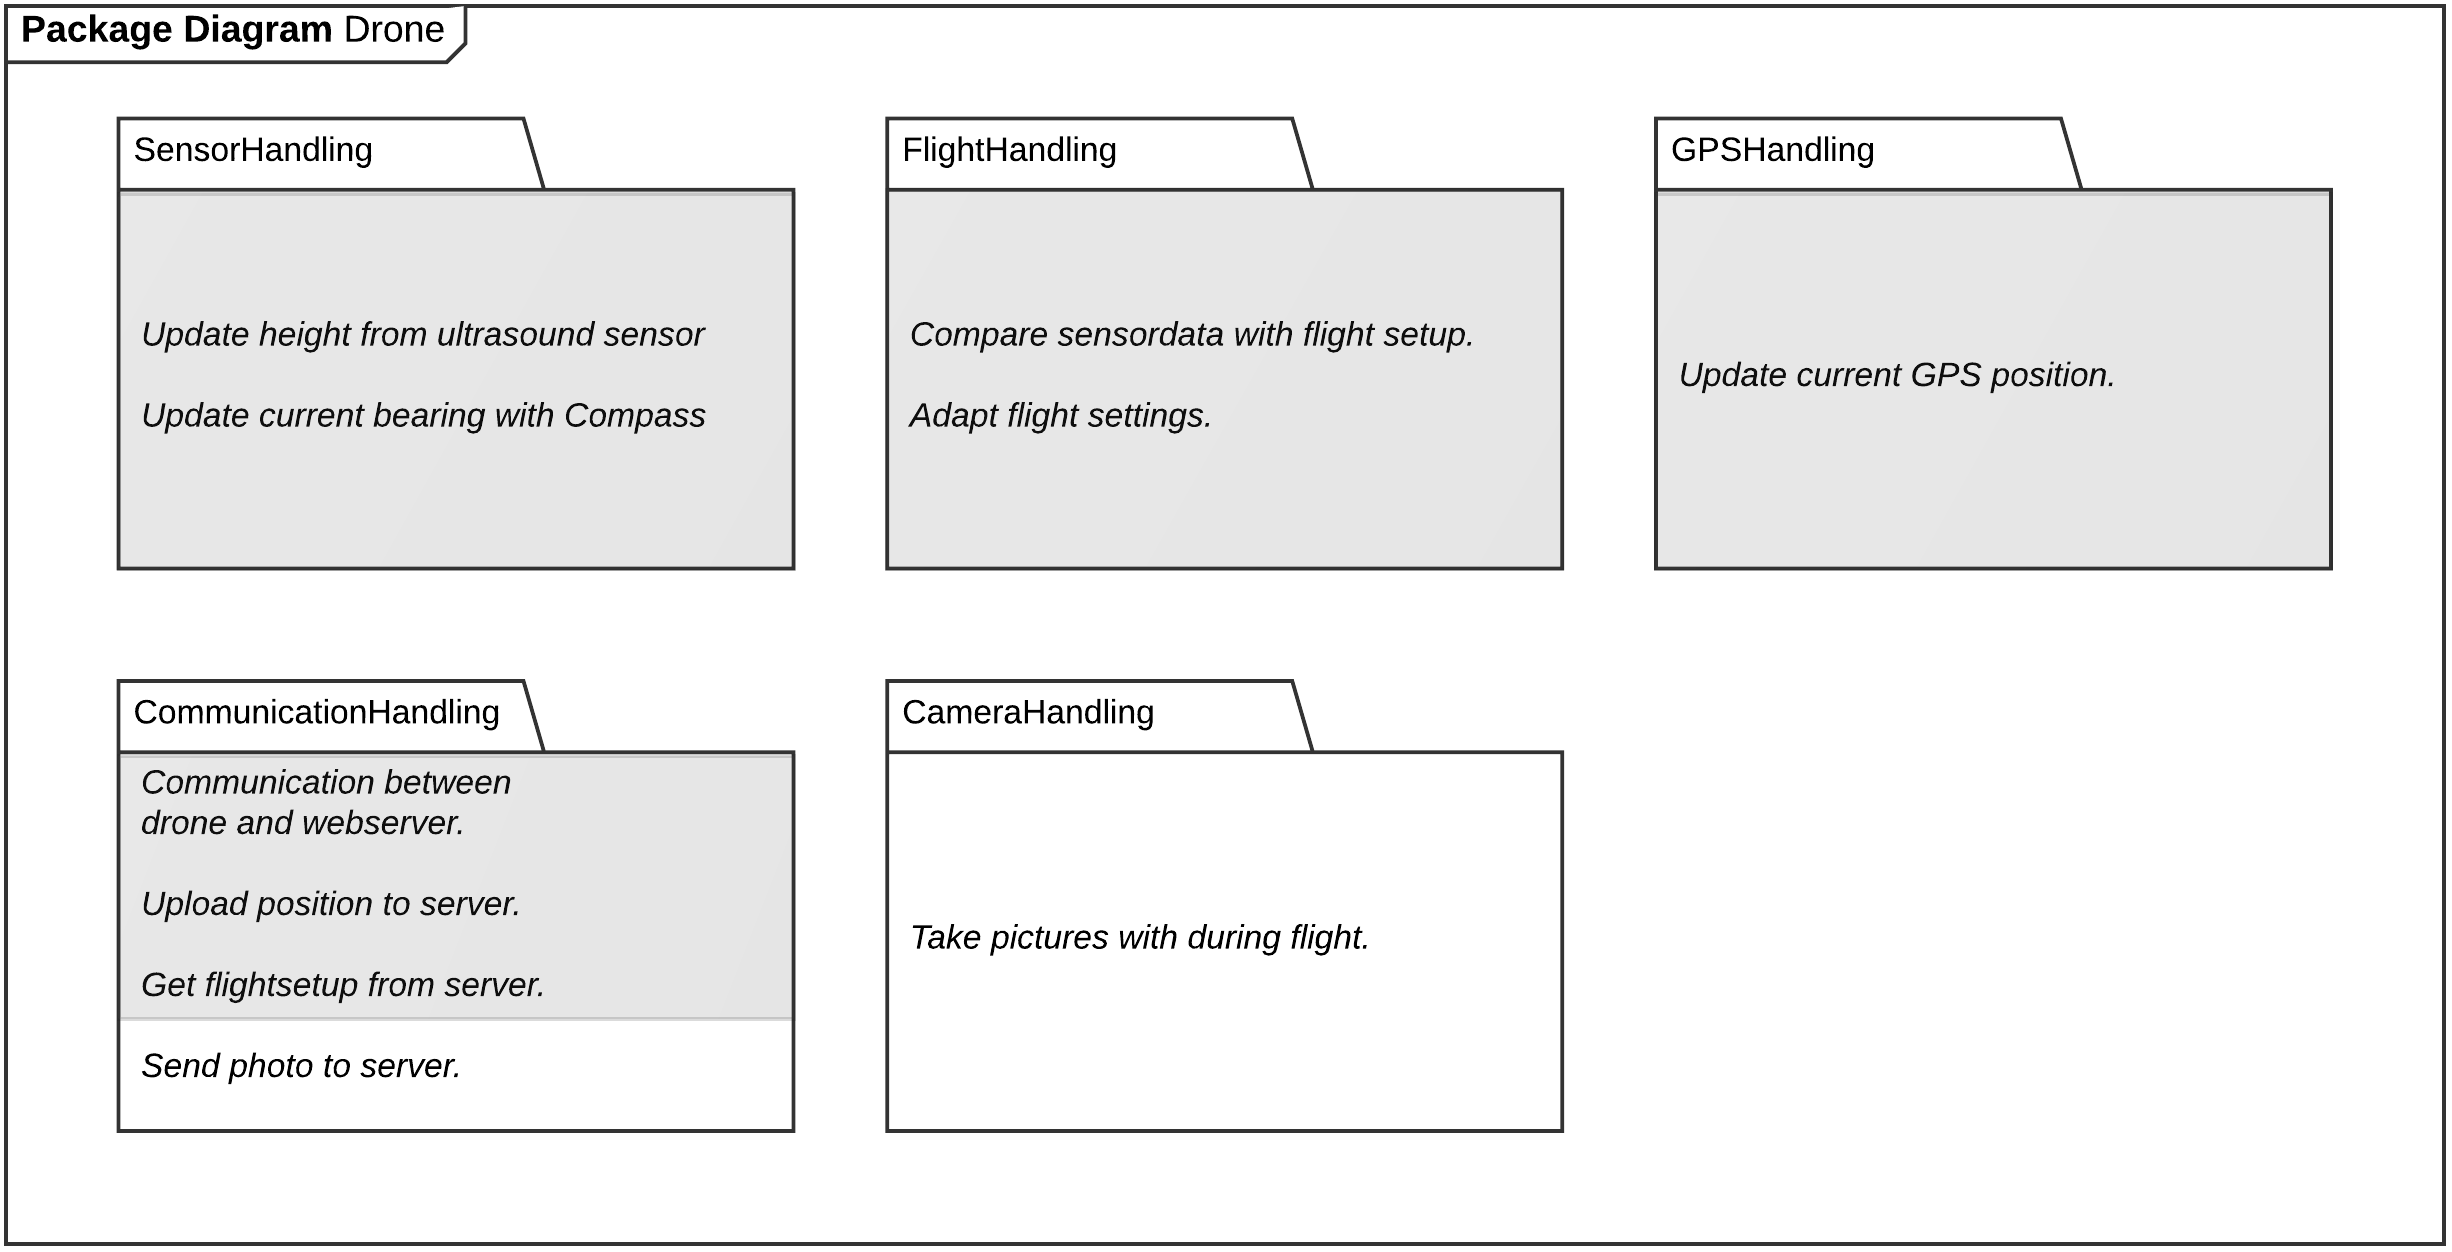
\includegraphics[width=1\textwidth]{Billeder/pakke_diagrammer/iteration3_drone.png}
	\vspace{-0.5cm}
	\caption{Pakkediagram drone}
	\label{fig:iteration2_pakke_diagram_drone}
\end{figure}

\textbf{SensorHandling}\\
Pakken er ansvarlig for indsamling af sensor data. I denne iteration skal pakken bruges til aflæsning af højdemåler og kompasset på flight control boardet. 

\textbf{FlightHandling}\\
Pakkens ansvar er kontrol og styring af drone under flyvning. Ved sammenligning af sensor data og data fra flyveopsætning tilpasses flyvehøjde, orientering mm

\textbf{GPSHandling}\\
Pakkens ansvar er håndtering af GPS. Dels er pakken ansvarlig for opstart og initiering af GPS, og desuden bruges pakken hver gang dronens nuværende GPS position skal opdateres.

\textbf{CommunicationHandling}\\
Pakkens ansvar er kommunikation imellem drone og server. Efter denne iteration skal dronen kunne hente flyveopsætninger fra server, sende sin nuværende GPS position til server og sende billeder til server.

\textbf{CameraHandling}\\
Pakkens ansvar er håndtering af kamera. Pakken bruges til at starte, initierer, bruge og slukke kameraet.


\newpage
\subsubsection*{Pakkediagram webapplikation}
I dette afsnit vises pakkediagram tilhørende webapplikation. Hver pakke i pakkediagrammet består af en eller flere klasser, der med stort samspil udfører opgaver indenfor et fælles ansvarsområde. 
På hver pakke findes en lille beskrivelse, der tydeliggør pakkens ansvarsområde.

\begin{figure}[H]
	\centering
	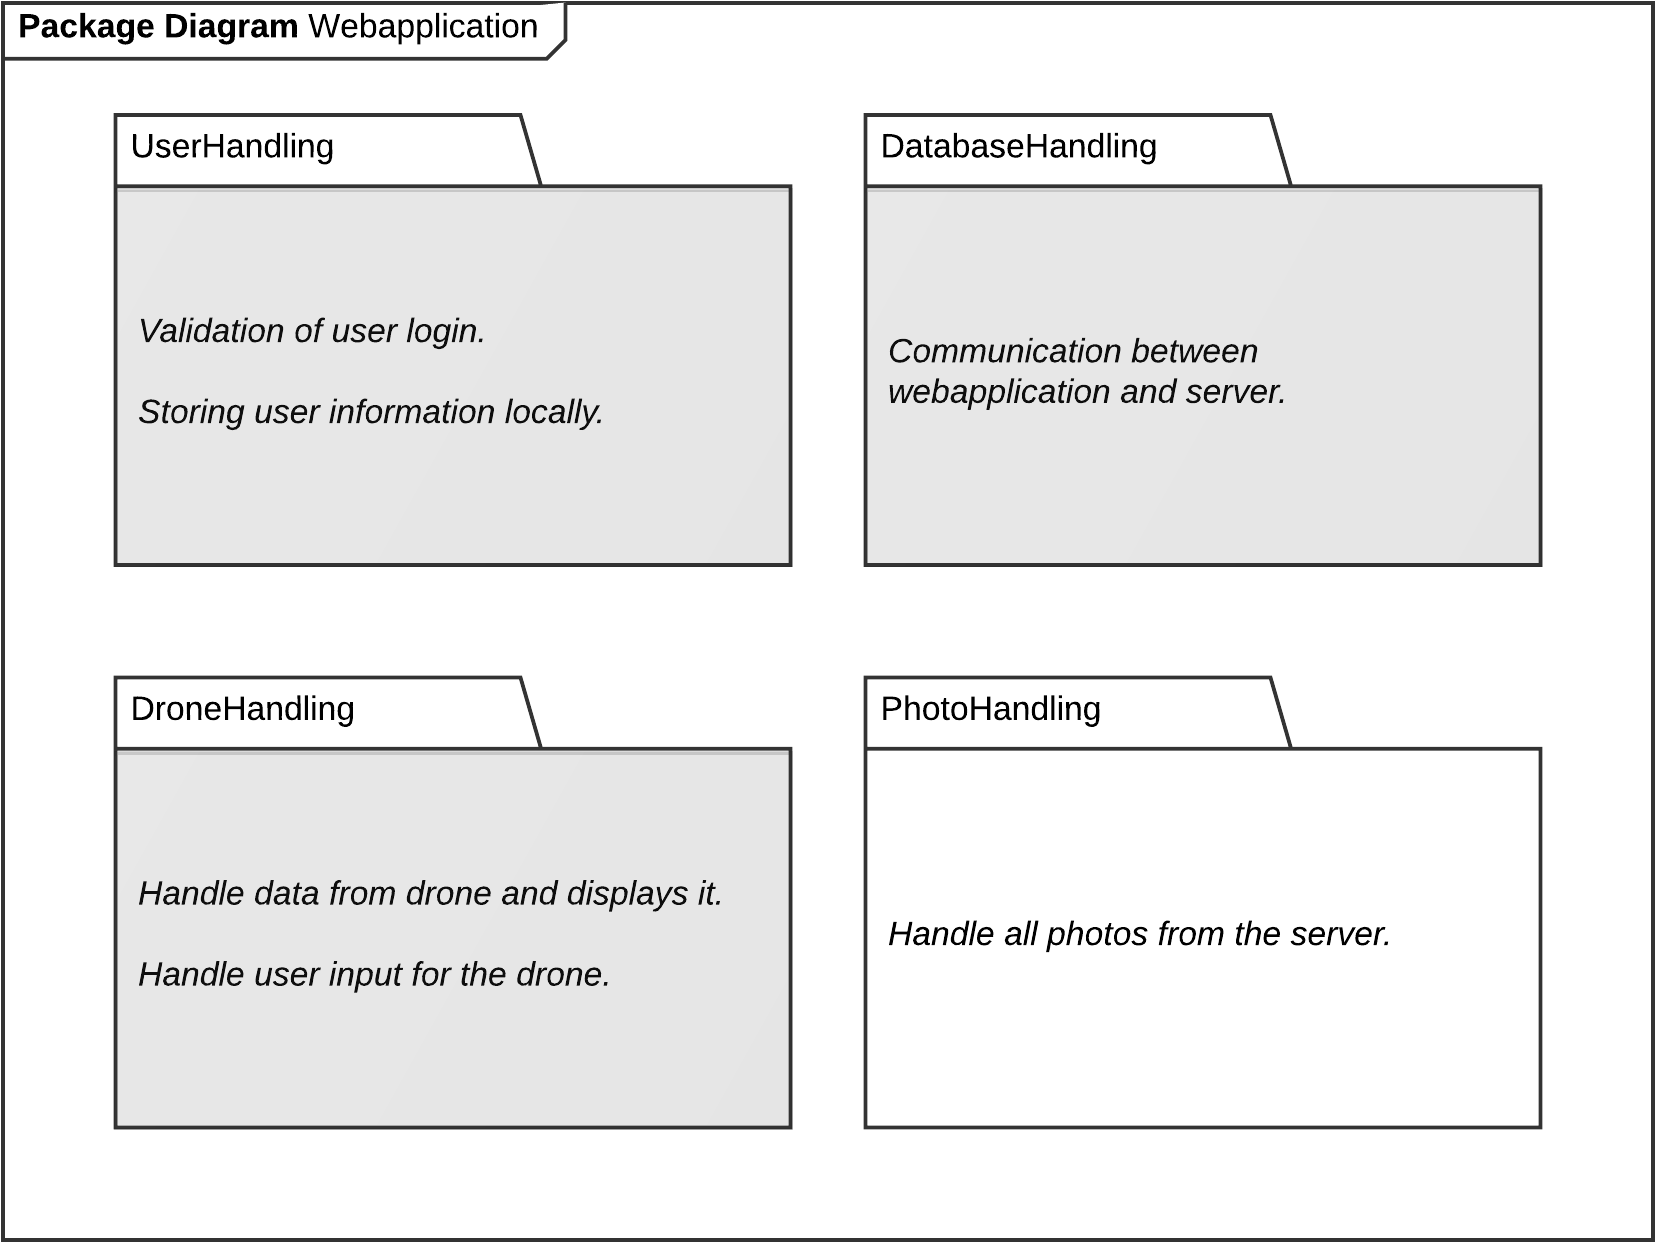
\includegraphics[width=1\textwidth]{Billeder/pakke_diagrammer/iteration3_server.png}
	\vspace{-0.5cm}
	\caption{Pakkediagram webapplikation}
	\label{fig:iteration3_pakke_diagram_webapplikation}
\end{figure}

\textbf{UserHandling}\\
Pakkens ansvar er validering af login/log ud på webapplikationen. Pakken har også ansvaret for at hente og gemme data om brugeren.

\textbf{DatabaseHandling}\\
Pakkens ansvar er kommunikation imellem databasen og serveren. 

\textbf{DroneHandling}\\
Pakken er ansvarslig for håndtering af events, waypoints og forskellige droner.

\textbf{PhotoHandling}\\
Pakkens ansvar er at håndtere de billeder dronen har taget under flyvning, præsentere dem for brugeren og sende dem videre i systemet.

\newpage

\subsubsection*{Sekvens diagram}
\vspace{-0.3cm}
På sekvensdiagrammet på figur \ref{fig:Sekvens_diagram_iteration3}, vises hvilke klasser der indgår og bruges i tredje iteration. På sekvensdiagrammet vises det, hvordan kamera delen af 3G/GPS modulet håndteres og hvordan nye billeder sendes via en post request til serveren. 

\vspace{-0.2cm}
%kommentar
\begin{figure}[H]
	\centering
	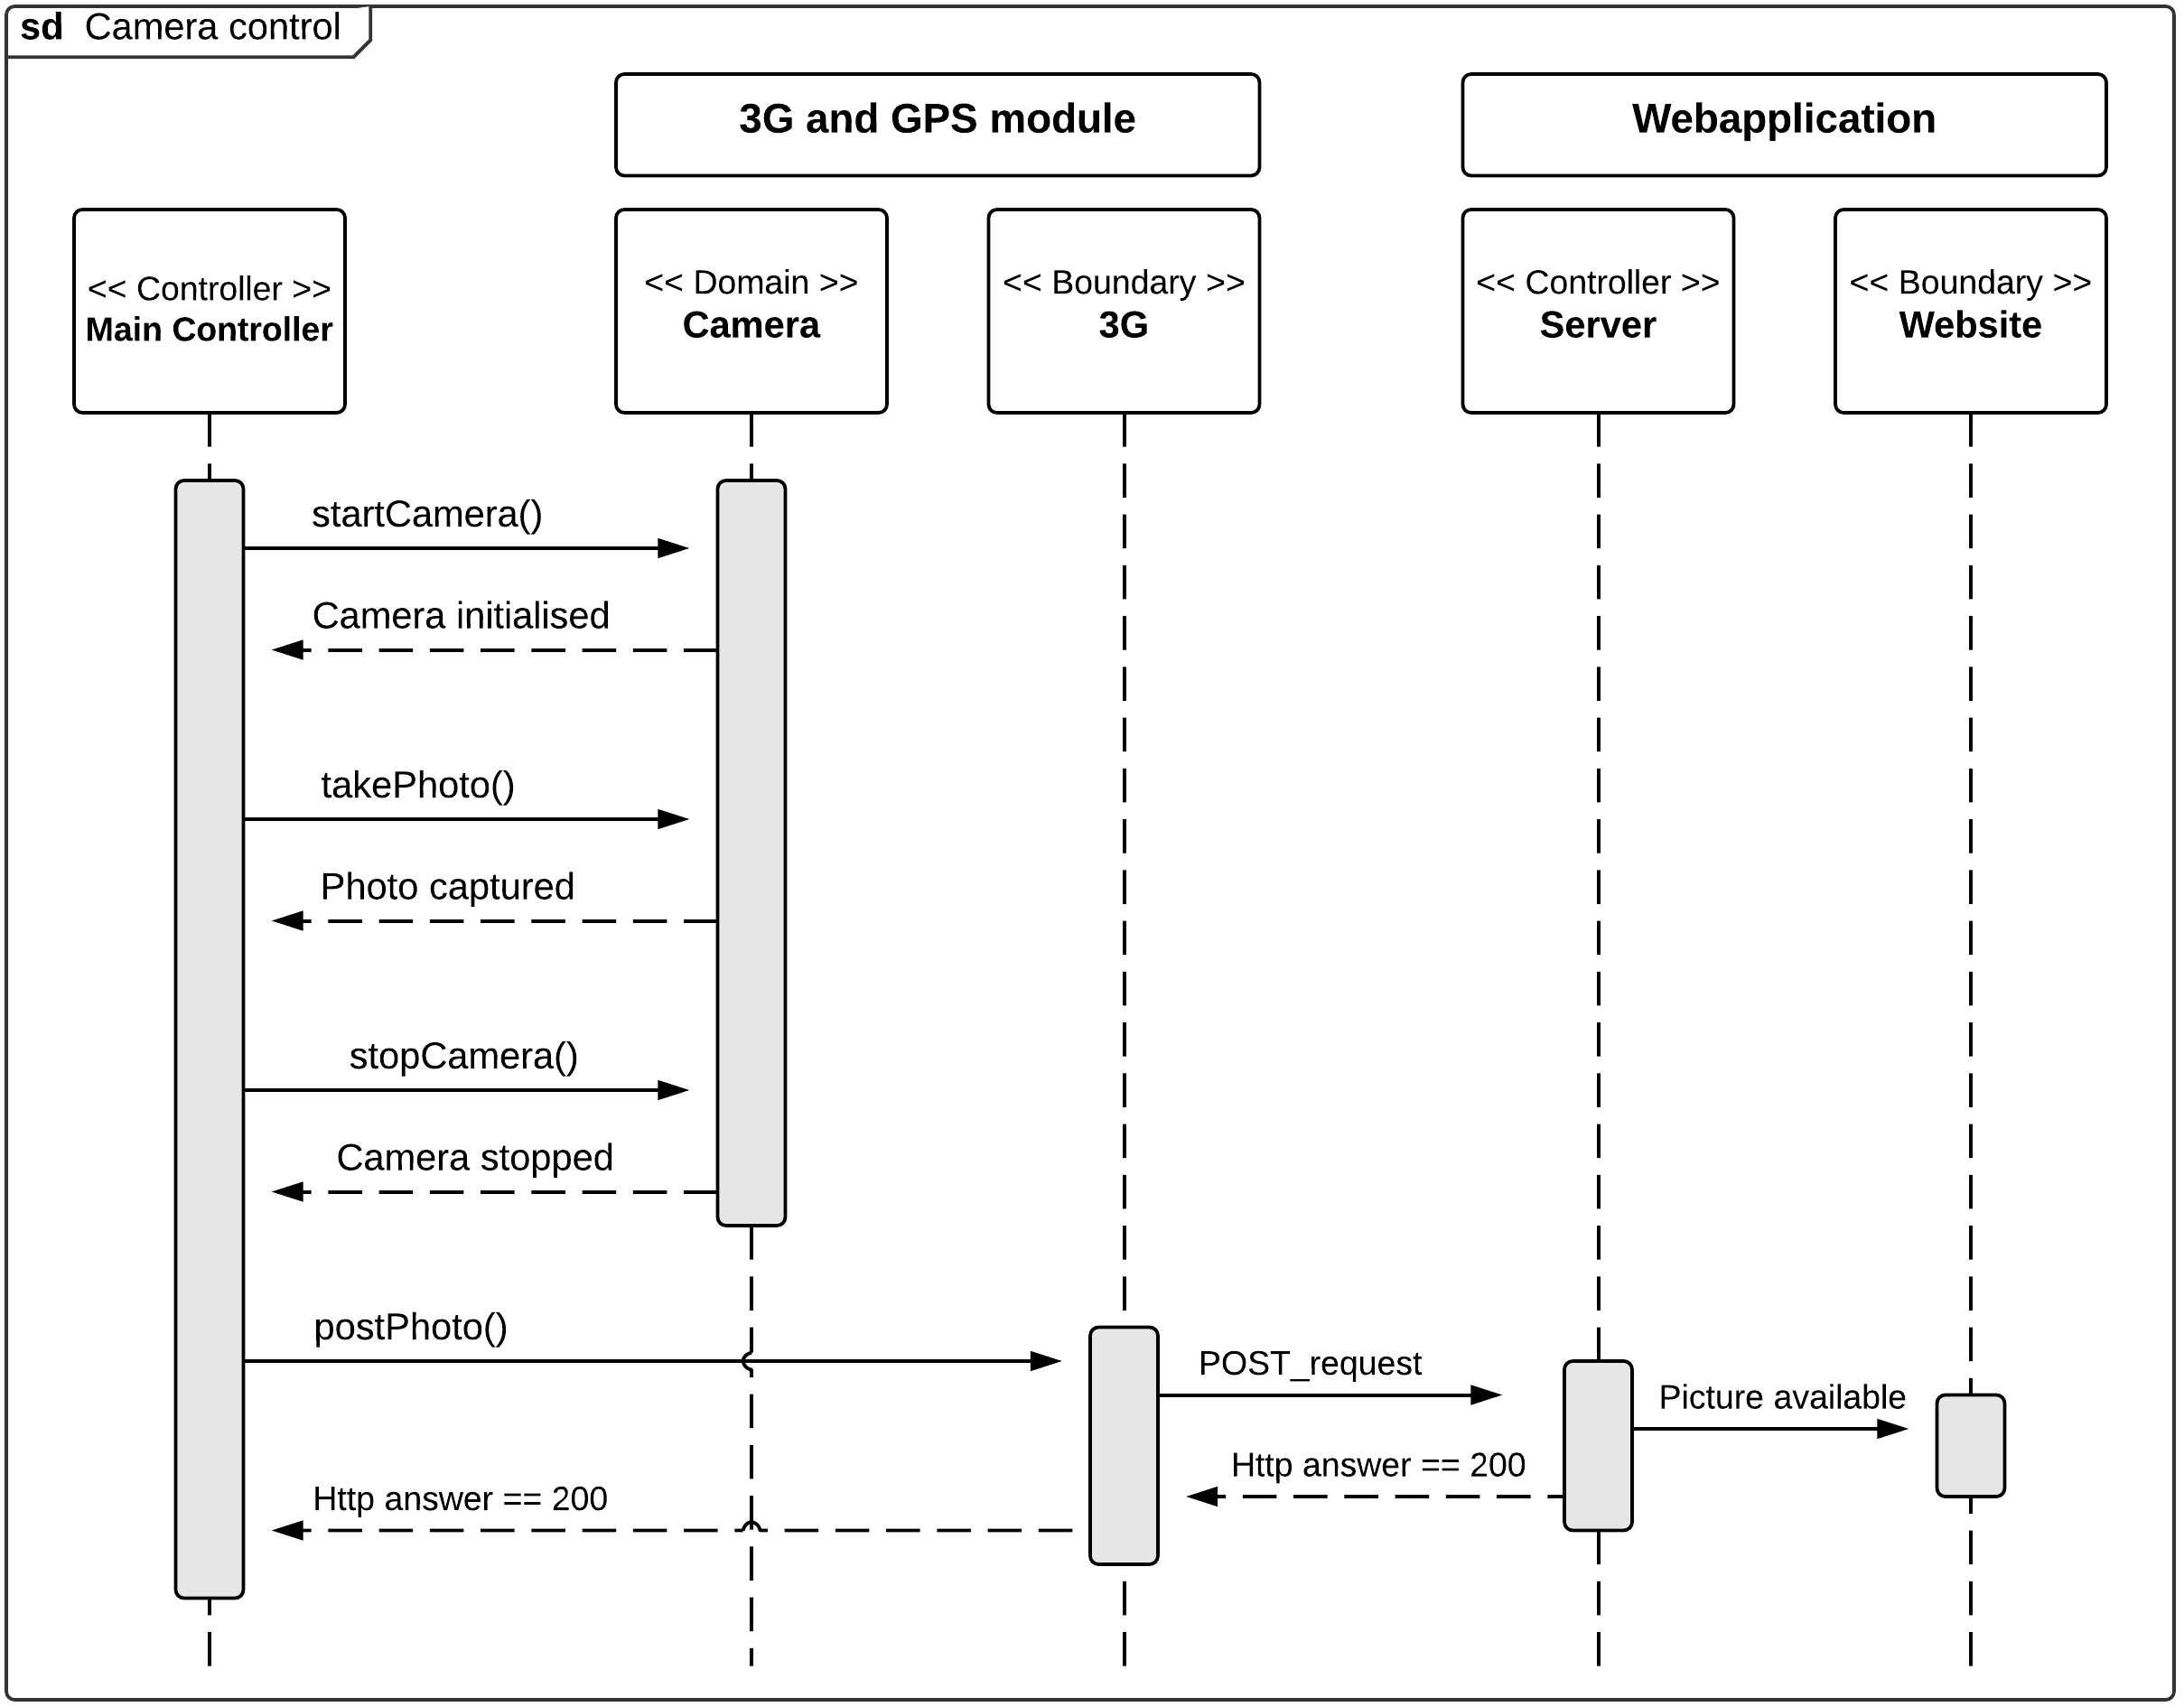
\includegraphics[width=1\textwidth]{Billeder/sekvens/sekvens_iteration3}
	\caption{Sekvens diagram \#iteration 3}
	\label{fig:Sekvens_diagram_iteration3}
\end{figure}
\vspace{-0.2cm}

\newpage

\subsubsection*{Klassediagram drone}

Figur \ref{fig:classDiagram_iteration3} viser et klassediagram tilhørende iteration 3. Klassediagrammet viser foruden main.cpp filen den nye Camera klasse og de nye metoder i Communication klassen.

%kommentar
\begin{figure}[H]
	\centering
	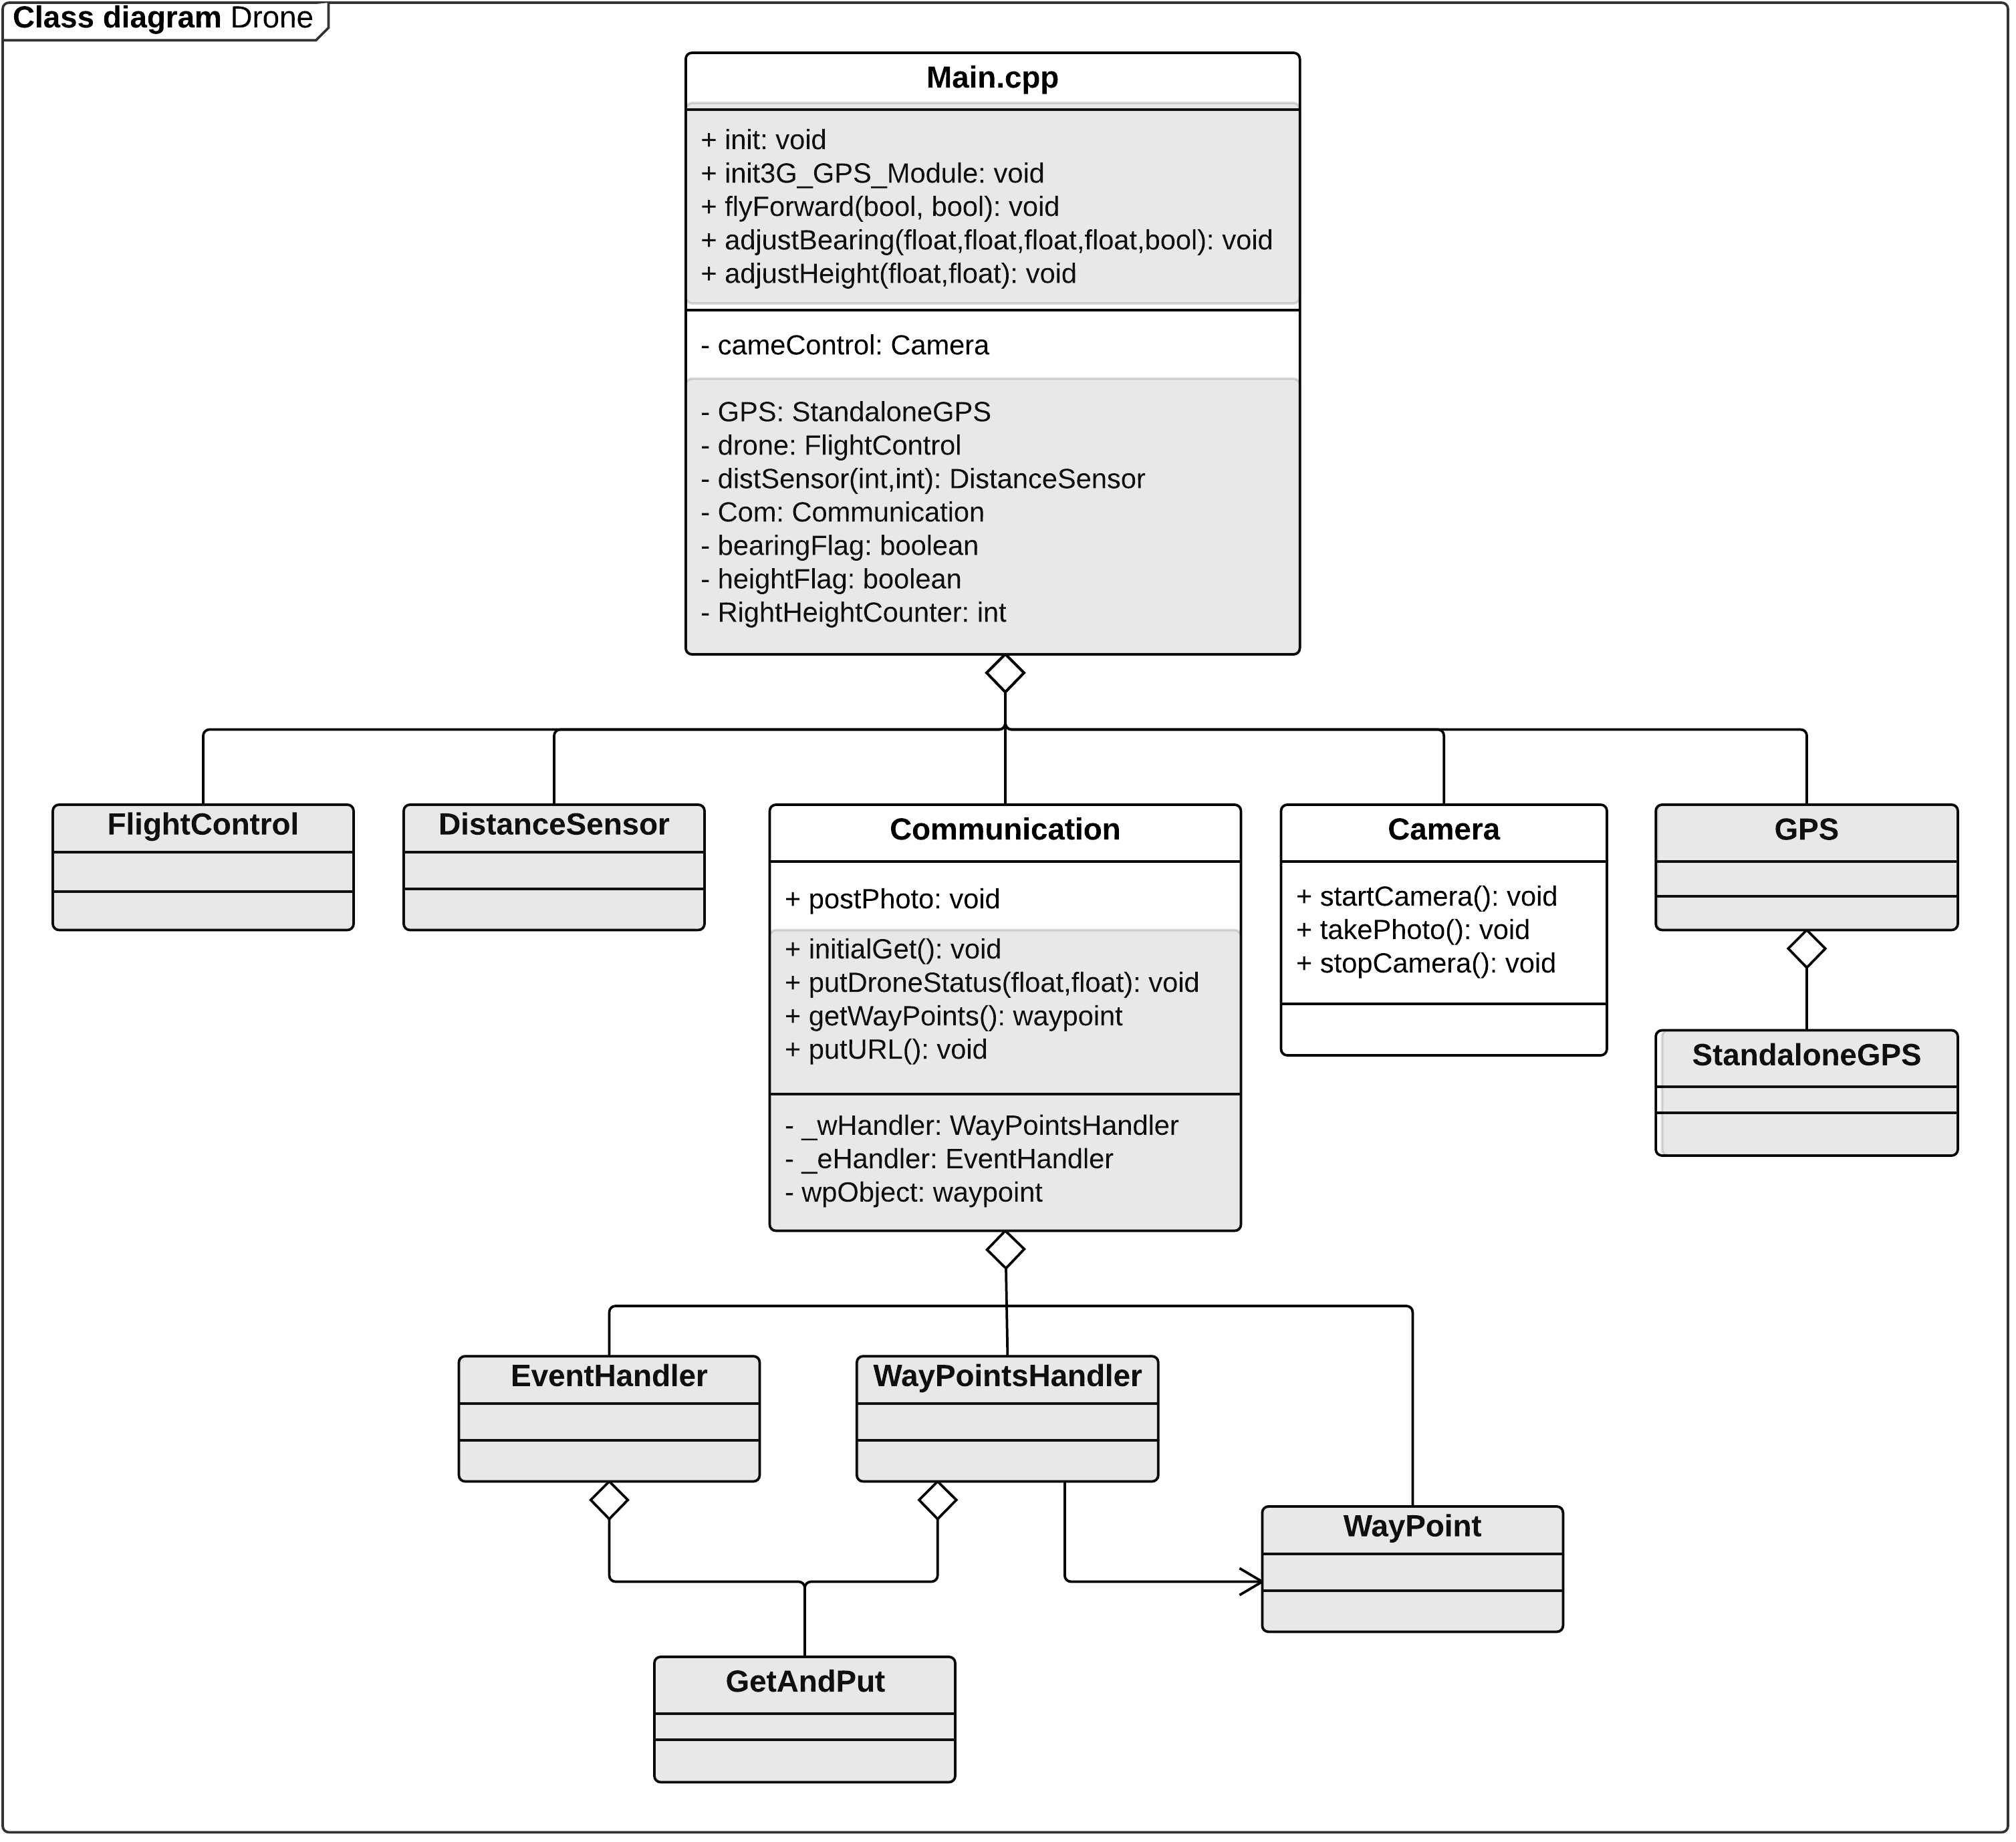
\includegraphics[width=1\textwidth]{Billeder/klasse_diagrammer/classdiagram_iteration3_drone.png}
	\vspace{-0.5cm}
	\caption{Klassediagram \#iteration 3}
	\label{fig:classDiagram_iteration3}
\end{figure}


\textbf{Camera} \\
Camera klassen er ansvarlig for at tage billeder og sende dem videre i systemet. 

\textbf{FlightControl} \\
FlightControl klassen står for alt styring af dronen. Bla. står FlightControl for kalibrering og styring af motorerne, samt aflæsning af højdesensor, GPS og kompas. 

\textbf{DistanceSensor} \\
DistanceSensor klassen bruges til at kontrollere de sensorer der er monteret på dronen. DistanceSensor klassen bruges udelukkende til kontrol af sensore til højdemåling. 

\newpage

\textbf{WayPointsHandler} \\
WayPointsHandler klassen håndterer de waypoints der hentes ned fra server. Klassen tager de hentede waypoints og gør dem tilgængelige for main.cpp. WayPointsHandleren gør brug af set-metoder fra WayPoint klassen.

\textbf{WayPoint} \\
WayPoint klassen bruges til at hente waypoints.  

\textbf{Main.cpp} \\
Main.cpp filen bruges til at sætte arduino board korrekt op, bla. sættes baudrate på de forskellige serielle forbindelser. Desuden bruges Main.cpp til at kalde og eksekverer forskellige klasse, objekter og funktioner. 

\textbf{GPS} \\
GPS klassen er implementeret som en abstract klasse. Init og updateGPSPosition er lavet som virtuelle metoder, hvilket betyder de skal implementeres i alle afledte klasser. GPS klassen er lavet fordi 3G/GPS modulet kunne bruges i 3 forskellige GPS modes. 

\textbf{StandaloneGPS}\\
Denne klasse er ansvarlig for al kommunikation med GPS'en når standalone mode er valgt. 

\textbf{GetAndPut} \\
GetAndPut klassen er den klasse der er tættest på hardwaren. Klassen indeholder http metoder der bruges til kommunikation mellem dronen og serveren. 

\textbf{Communication} \\
Communication klassen styrer alt der har med 3G kommunikation at gøre.

\textbf{EventHandler} \\
EventHandler klassen håndterer Events, og bruges som bindeled mellem communication- og GetAndPut klassen. EventHandleren sorterer eventID'et fra data der modtages og returnerer værdien af eventID til communication klassen. 




\newpage

\subsubsection*{Klassediagram webapplikation}

På figur \ref{fig:classDiagram_iteration3} vises klassediagrammet tilhørende iteration 3. 

%kommentar
\begin{figure}[H]
	\centering
	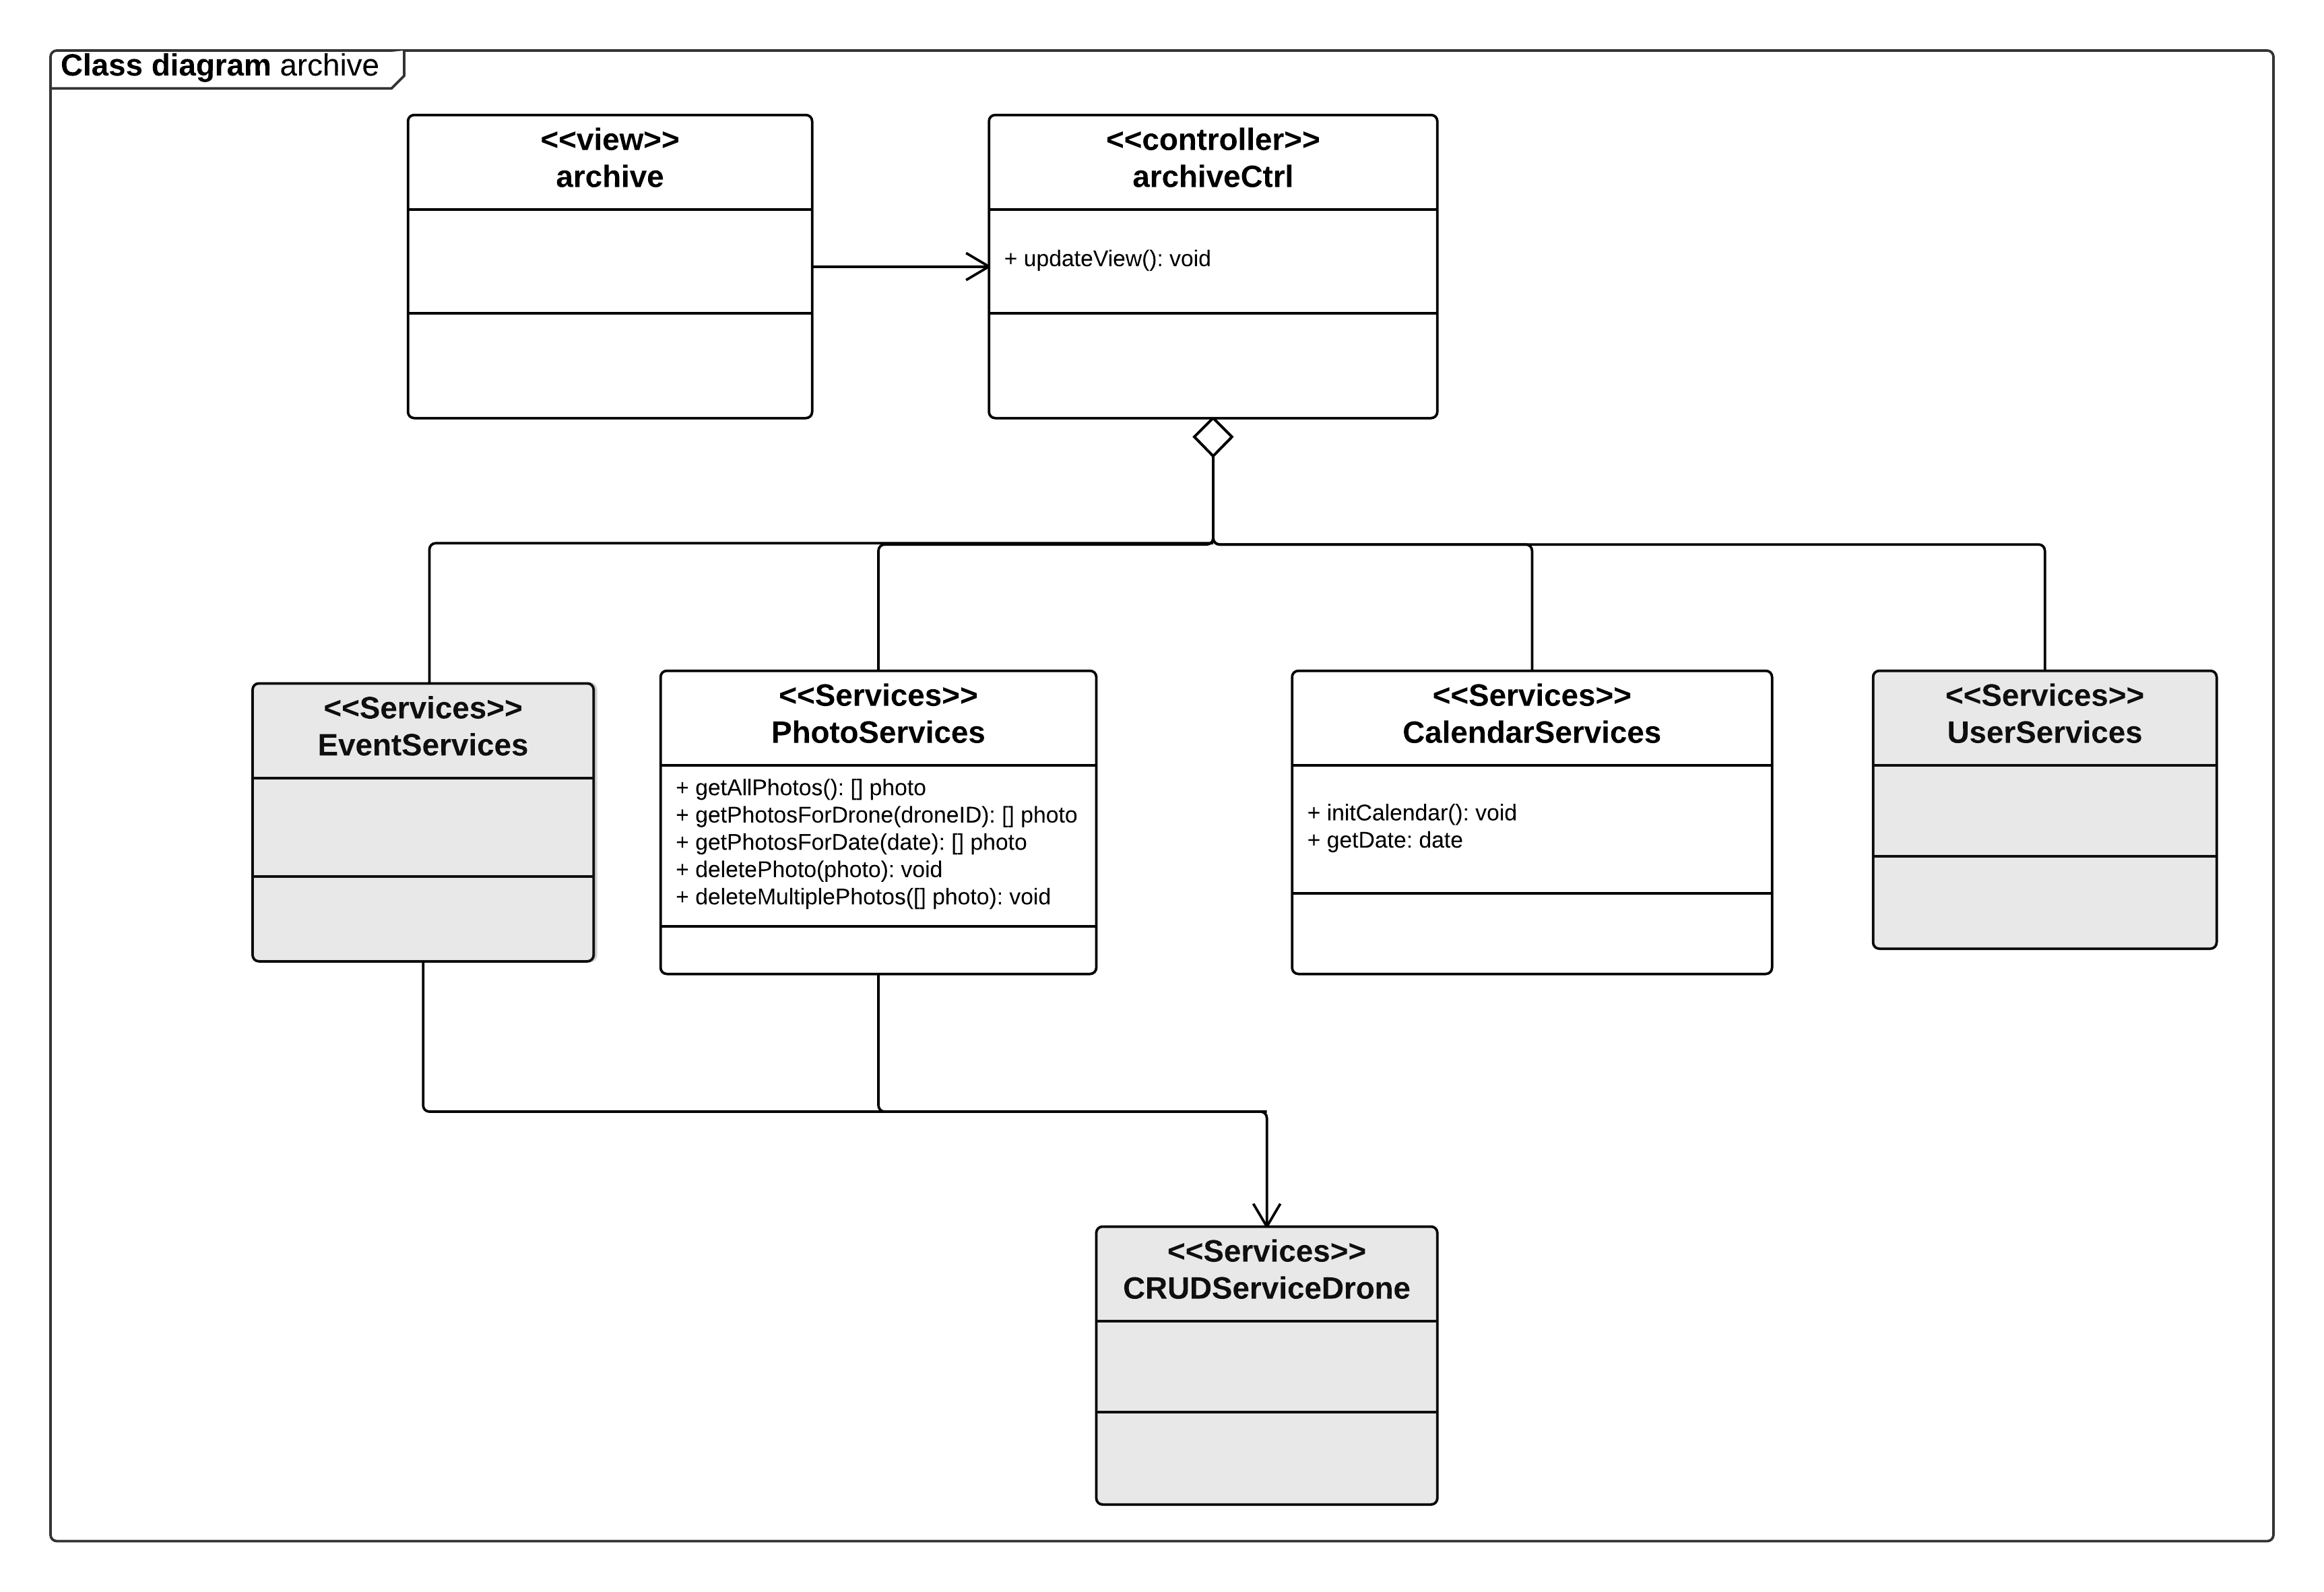
\includegraphics[width=1\textwidth]{Billeder/klasse_diagrammer/classdiagram_iteration3_server.png}
	\vspace{-0.5cm}
	\caption{Klassediagram \#iteration 3}
	\label{fig:classDiagram_iteration3}
\end{figure}

\textbf{archive}\\
Denne klasse håndterer view'et tilhørende iteration tre. Sammen med archiveCtrl skaber archive klassen det bruger ser i sin browser.

\textbf{archiveCtrl}\\
ArchiveCtrl klassen er controller klassen til iteration tre. Det er den eneste klasse der har direkte forbindelse til view klassen. ArchiveCtrl klassen deler hukommelse med view'et igennem two-way-binding med scopes.

\textbf{EventServices}\\
Denne klasse indeholder logikken om event håndtering. Klassen bruges til at hente en event liste, et enkelt event for en givet drone og sende et nyoprettet event til serveren via CRUDServiceDrone klassen.

\textbf{PhotoServices}\\
Denne klasse indeholder logikken om foto håndtering. Klassen bruges til at hente fotos via CRUDServiceDrone klassen, derudover har klassen ansvaret for at slette uønskede billeder.
\newpage

\textbf{CalendarServices}\\
Denne klasse indeholder logikken for kalenderen, klassen bruges til at oprette og navigere i kalenderen. Desuden bruges klassen til at fortælle hvilken dato der er valgt, når  billeder fra tidligere flyvning ønskes vist.

\textbf{UserServices}\\
UserServices bruges til at gemme information om hvilken bruger der er logget ind i systemet.

\textbf{CRUDServicesDrone}\\
Denne klasse bruges som bindeled imellem server og webapplikation, og indeholder logik til serveren. CRUDServicesDrone bruges når der sendes Get, Put og Post til serveren.


\vspace{0.3cm}

\subsubsection*{State machine diagram}
\vspace{-0.3cm}
I state machine diagrammet på figur \ref{fig:Statemachine_iteration3}, vises hvordan flowet i systemet er. Der er tilføjet en enkelt state, der håndterer alt det der har med billeder at gøre. 

\vspace{-0.2cm}
%kommentar
\begin{figure}[H]
	\centering
	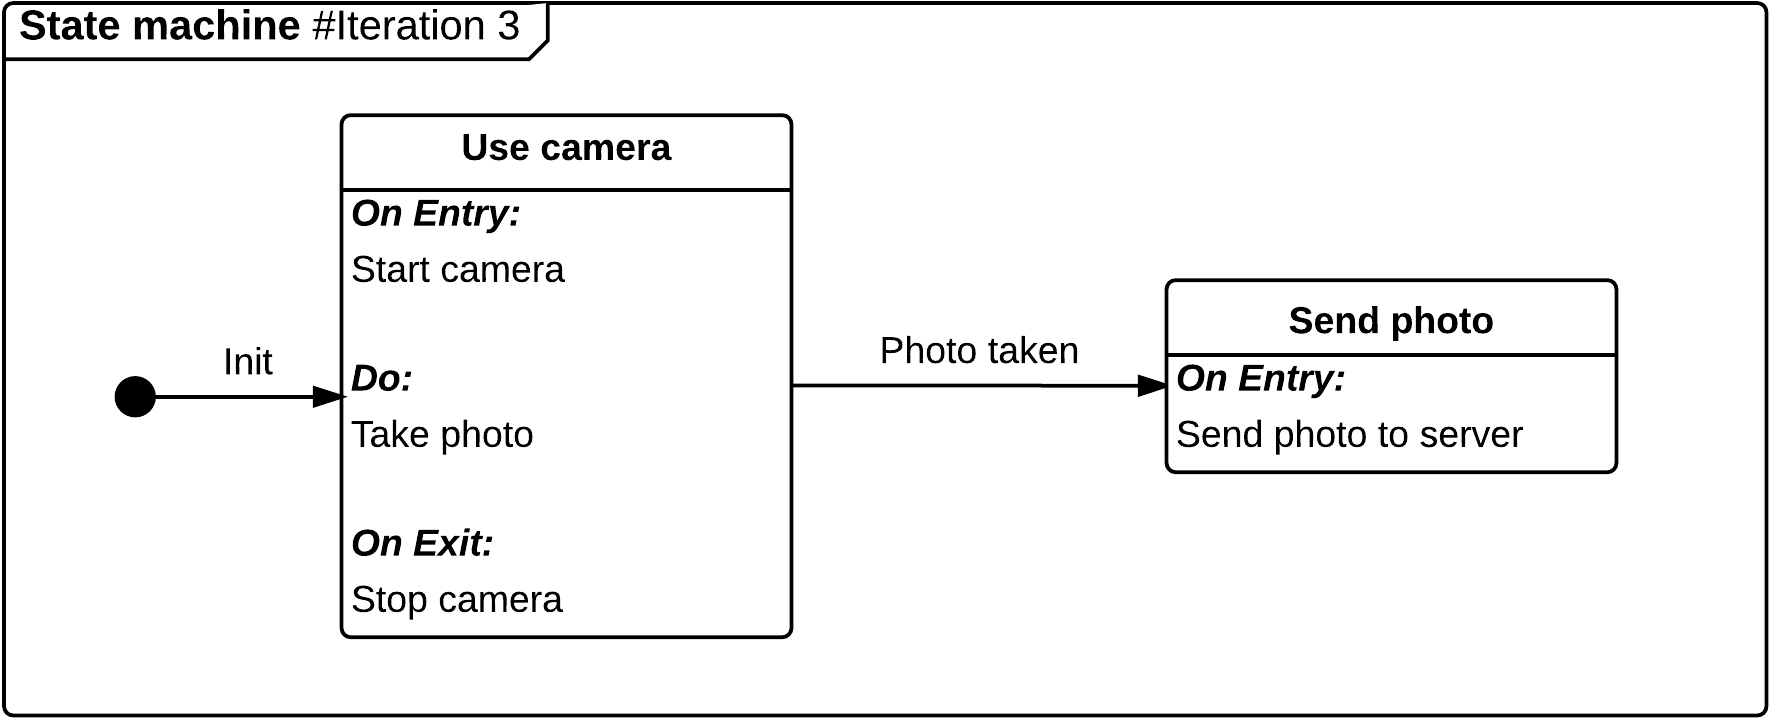
\includegraphics[width=1\textwidth]{Billeder/statemachine/State_iteration3.png}
	\caption{State machine \#iteration 3}
	\label{fig:Statemachine_iteration3}
\end{figure}

